%! Author = Len Washington III
%! Date = 9/27/24

% Preamble
\documentclass[
	number={6},
	title={Clustering}
]{cs584notes}

% Document
\begin{document}

\section{Clustering}\label{sec:clustering}
\emph{Clustering} is an \emph{unsupervised learning} technique which automatically \emph{partitions unlabeled data} into groups of \emph{similar datapoints}.
It is useful for:
\begin{description}[font=\emph]
	\item[Segmentation] Segmenting a large set of cases into small subsets that can be treated similarly.
	\begin{itemize}
		\item e.g., image segmentation.
	\end{itemize}
	\item[Compression] Generate a more compact description of a dataset.
	\begin{itemize}
		\item e.g., handwritten digit recognition.
	\end{itemize}
	\item[Representation] Model an underlying process that generates the data as a mixture of different, localized processes.
\end{description}

\section{Clustering Applications}\label{sec:clustering-applications}
\begin{itemize}
	\item Cluster news articles or web pages or search results by topic.
	\item Cluster protein sequences by function of genes according to expression profile.
	\item Cluster users of social networks by interest.
	\item Cluster galaxies or nearby stars.
\end{itemize}

\section{Clustering Algorithms}\label{sec:clustering-algorithms}
\subsection{Flat clustering}\label{subsec:flat-clustering}
No inter-cluster structure.
\begin{itemize}
	\item $k$-means algorithm.
	\item Gaussian mixture models (GMM).
	\item Spectral clustering.
\end{itemize}

\subsection{Hierarchical clustering}\label{subsec:hierarchical-clustering}
Clusters for a hierarchy.
\begin{itemize}
	\item Bottom-up (agglomerative clustering).
	\item Top-down (divisive clustering).
\end{itemize}

\subsection{Hard clustering}\label{subsec:hard-clustering}
Items are assigned to a unique cluster.
\begin{itemize}
	\item $k$-means algorithm.
	\item Spectral clustering.
\end{itemize}

\subsection{Soft (fuzzy) clustering}\label{subsec:soft-clustering}
Cluster membership is a real-valued function, distributed across several clusters.
\begin{itemize}
	\item Soft $k$-means.
	\item Gaussian mixture models.
\end{itemize}

\subsection{Centroid-based clustering}\label{subsec:centroid-based-clustering}
This type of clustering algorithm forms around the \emph{centroids} of the data points.
E.g., $k$-means, $k$-modes.

\subsection{Distribution-based clustering}\label{subsec:distribution-based-clustering}
Clustering algorithm is modeled using statistical \emph{distributions}.
It assumes that the data points in a cluster are generated from a particular \emph{probability distribution}, and the algorithm aims to estimate the parameters of the distribution.
E.g., GMM\@.

\subsection{Density-based clustering}\label{subsec:density-based-clustering}
This type of clustering algorithm groups together data points that are in \emph{high-density concentration} and separates points in \emph{low-concentration} regions.
E.g., DBSCAN\@.

\section{$k$-Means Clustering}\label{sec:k-means-clustering}
\begin{itemize}
	\item \emph{$k$-means algorithm} is an \emph{iterative clustering} algorithm, based on the Euclidean distance.
	It is a \emph{non-parametric} learning algorithm.
	\item A \emph{greedy algorithm} (Lloyd's algorithm) locally optimizes the \emph{cluster quality} measure:
	\begin{itemize}
		\item The \emph{cluster quality} measure is computed based on the \emph{cluster centroid}.
		\item Find the \emph{closest cluster center} for each item and assign it to that cluster.
		\item \emph{Recompute} the \emph{cluster centroid} as the mean of items, for the newly-assigned items in the cluster.
	\end{itemize}
\end{itemize}

\begin{figure}[H]
	\centering
	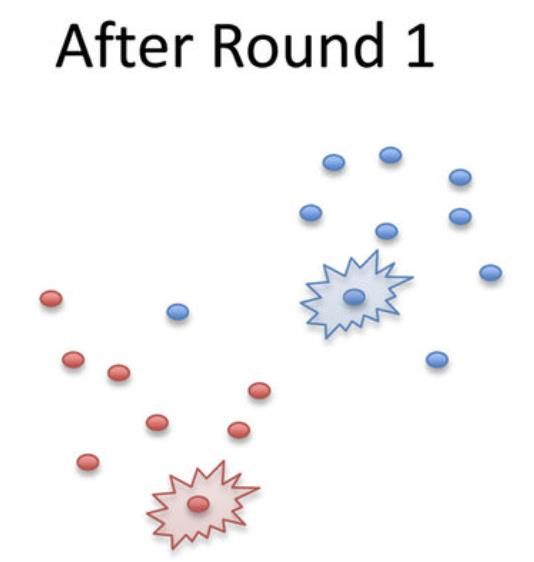
\includegraphics[width=\textwidth]{figures/6/k_means_example}
	\caption{$k$-Means Clustering}
	\label{fig:k-means-clustering}
\end{figure} % TODO: Add the other figures in a subfigure env

\begin{itemize}
	\item \emph{Initialize}: Pick \data{$k$} \emph{data} points as cluster \emph{centers}.
	\item \emph{Repeat}:
	\begin{itemize}
		\item \emph{Assign} data points to \emph{closest cluster center}.
		\item \emph{Change} the \emph{cluster center} to the \emph{average} of its assigned points.
	\end{itemize}
	\item \emph{Stop} when the \emph{assignments} of data points do \emph{not change}.
	\item \emph{Input}: A set of \data{$n$} \emph{datapoints} \data{$x_{1}, x_{2}, \dots, x_{n} \in \mathbb{R}^{d}$} with \data{$k$} \emph{clusters}.
	\item \emph{Output}: \data{$k$} representatives \data{$c_{1}, c_{2}, \dots, c_{k} \in \mathbb{R}^{d}$}.
	\item \emph{Objective}: choose \data{$c_{1}, c_{2}, \dots, c_{k} \in \mathbb{R}^{d}$} such that:
	\data{\begin{equation}
		\min\sum_{i=1}^{n}\sum_{j=1}^{k} || x_{i} - c_{j} ||^{2}
		\label{eq:k-means}
	\end{equation}}
	\item \emph{Initialize} cluster centers \data{$c_{1}, c_{2}, \dots, c_{k}$} and clusters \data{$C_{1}, C_{2}, \dots, C_{k}$}.
	\item \emph{Repeat} until there is no further change:
	\begin{itemize}
		\item For each \data{$j: C_{j} \gets \{ x \mbox{ \textcolor{black}{whose \emph{closest center} is }} c_{j} \}$}.
		\item For each \data{$j: c_{j} \gets \mbox{ \emph{mean} of } C_{j}$}.
	\end{itemize}
\end{itemize}

\begin{equation*}
\begin{aligned}
	\sum_{i=1}^{4}\sum_{j=1}^{2} ||x_{i} - c_{j}||^{2} &= ||x_{1} - c_{1}||^{2} + ||x_{1} - c_{2}||^{2} + ||x_{2} - c_{1}||^{2} + ||x_{2} - c_{2}||^{2} \\&+ ||x_{3} - c_{1}||^{2} + ||x_{3} - c_{2}||^{2} + ||x_{4} - c_{1}||^{2} + ||x_{4} - c_{2}||^{2}\\
	&= 0^{2} + 3^{2} + 1^{2} + 2^{2} + 2^{2} + 1^{2} + 0^{2} + 3^{2}\\
	&= 0 + 9 + 1 + 4 + 4 + 1 + 0 + 9\\
	&= 28
\end{aligned}
\end{equation*}

With updated cluster centers \data{$c_{1}$} and \data{$c_{2}$}, recompute the objective function:
\begin{equation*}
\begin{aligned}
	0.5^{2} + 2.5^{2} + 0.5^{2} + 1.5^{2} + 1.5^{2} + 0.5^{2} + 2.5^{2} + 0.5^{2}
	&= 0.25 + 6.25 + 0.25 + 2.25 + 2.25 + 0.25 + 6.25 + 0.25\\
	&= 18
\end{aligned}
\end{equation*}

% TODO: Figure out how to do figures

\subsection{$k$-Means Properties}\label{subsec:$k$-means-properties}
\begin{itemize}
	\item It is guaranteed to \emph{converge} is a finite number of iterations, but it may converge at a \emph{local optimum} that is different from the global optimum.
	\item \emph{Initialization} is crucial as it \emph{decides} how fast it \emph{converges} as well as the quality of the solution output.
	\item Time complexity: \data{$O(kdni)$}
	\begin{description}[font=\data]
		\item[$n$] the number of \data{$d$}-dimensional \emph{data} (to be clustered).
		\item[$k$] the number of \emph{clusters}.
		\item[$i$] the number of \emph{iterations} needed until \emph{convergence}.
	\end{description}
\end{itemize}

% TODO: More figures

\section{Furthest Point Initialization}\label{sec:furthest-point-initialization}
\begin{itemize}
	\item Choose \data{$c_{1}$} arbitrarily at random.
	\item For \data{$j=2, \dots, k$}
	\begin{itemize}
		\item \emph{Pick} \data{$c_{j}$} among the datapoints \data{$x_{1}, x_{2}, \dots, x_{n}$} that is \emph{farthest} from the \emph{previously chosen cluster centers} \data{$c_{1}, c_{2}, \dots, c_{j-1}$}.
	\end{itemize}
	\item This method solves the \emph{issues} with random initialization pertaining to \emph{well separated clusters}.
	\item However, this method of initialization is \emph{sensitive} to outliers.
\end{itemize}

\section{Pros and Cons}\label{sec:k-means-pros-and-cons}
Pros:
\begin{itemize}
	\item Easy to implement.
	\item Guarantees convergence.
	\item Generalized to clusters of different shapes and sizes.
\end{itemize}
Cons:
\begin{itemize}
	\item Choosing a $k$ manually.
	\item Final solution is dependent on initial values.
	\item Curse of dimensionality.
\end{itemize}

\begin{figure}[H]
	\centering
	\begin{subfigure}{0.475\textwidth}
		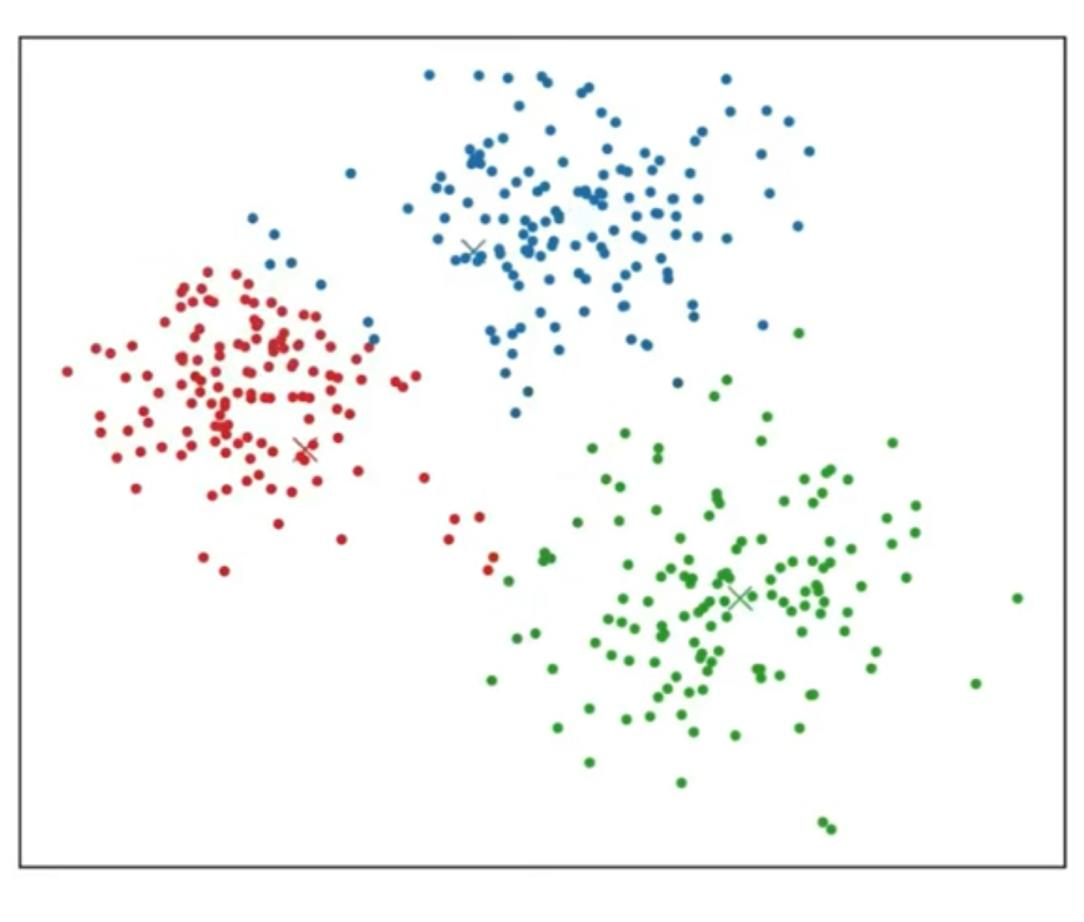
\includegraphics[width=\textwidth]{figures/6/k_means}
		\caption{$k$-means}
		\label{fig:k-means}
	\end{subfigure}\hfill
	\begin{subfigure}{0.475\textwidth}
		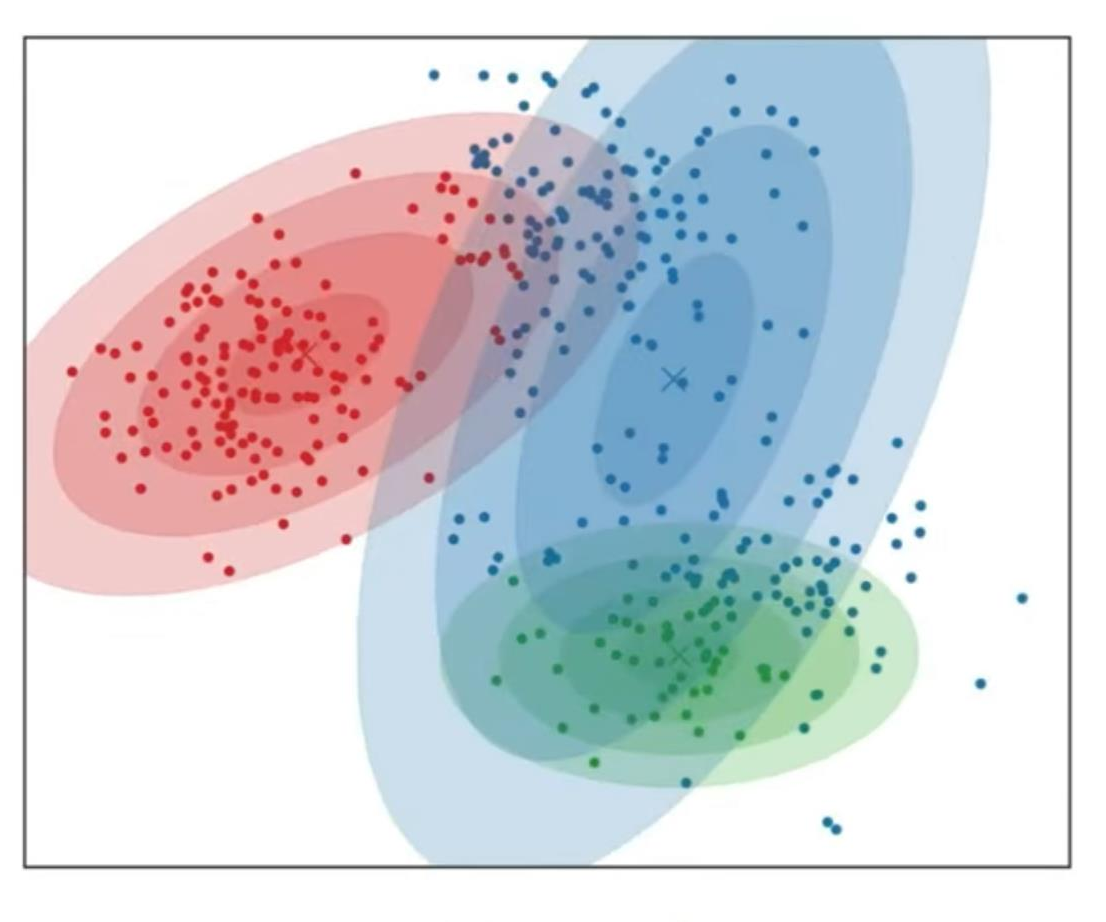
\includegraphics[width=\textwidth]{figures/6/gmm}
		\caption{GMM}
		\label{fig:gmm}
	\end{subfigure}
	\caption{$k$-Means vs. GMM}
	\label{fig:k-means-vs-gmm}
\end{figure}

\section{Gaussian Mixture Models (GMMs)}\label{sec:gaussian-mixture-models-(gmm)s}
\begin{itemize}
	\item \emph{Clusters} are models as \emph{gaussian} i.e., the data within a cluster follows the normal or \emph{\hyperref[eq:gaussian-distribution]{gaussian distribution}}:
	\begin{equation}
		N(x | \mu, \sigma) = \frac{1}{\sqrt{2\pi\sigma}}e^{\left( -\frac{1}{2}\frac{(x-\mu)^{2}}{\sigma} \right)}
		\label{eq:gaussian-distribution-2}
	\end{equation}
	\item The \emph{GMM clustering} approach uses:
	\begin{itemize}
		\item Parametric learning
		\item Probabilistic learning
		\item Generative learning
	\end{itemize}
	\item \emph{Expectation-Maximation (EM) algorithm} assigns data points to a cluster with some probability.
\end{itemize}

\begin{figure}[H]
	\centering
	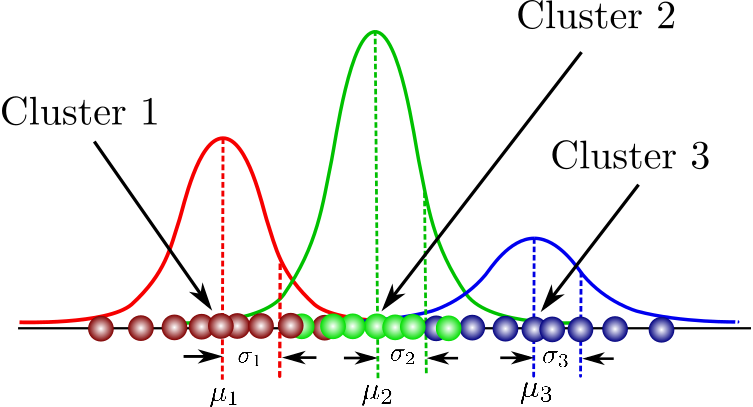
\includegraphics[width=\textwidth]{figures/6/gmm_clusters}
	\caption{Gaussian Mixture Models}
	\label{fig:gmm-clusters}
\end{figure}

\begin{figure}[H]
	\centering
	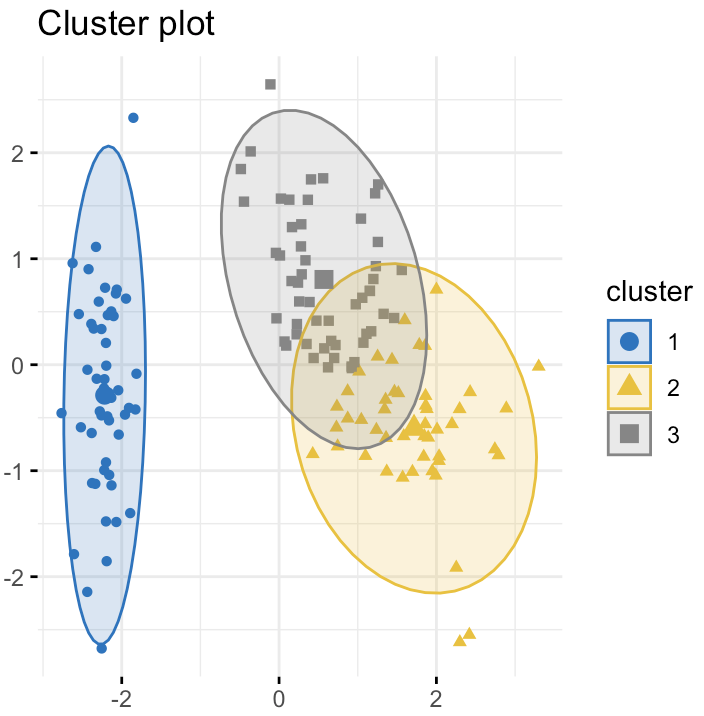
\includegraphics[width=\textwidth]{figures/6/gmm_cluster_plot}
	\caption{GMM Cluster Plot}
	\label{fig:gmm-cluster-plot}
\end{figure}

\begin{itemize}
	\item \emph{Likelihood} is the \emph{probability} of \emph{observing} the \emph{data} given the parameters of the model.
	In the \emph{EM algorithm}, the goal is to \emph{find} the \emph{parameters} that \emph{maximize the likelihood}.
	\item Latent Variables are \emph{unobserved variables} in statistical models that can only by \emph{inferred indirectly} through their effects on observable variables.
	\item \emph{Parameters (latent variables) describing a \emph{cluster} \data{$c$}}:
	\begin{description}[font=\data]
		\item[$\mu_{c}$] Mean
		\item[$\sigma_{c}$] Covariance
		\item[$\pi_{c}$] Weight
	\end{description}
\end{itemize}

\section{GMM Probability}\label{sec:gmm-probability}
\begin{equation}
	P(x) = \sum_{c=1}^{k} \pi_{c} N(x | \mu_{c}, \sigma_{c})
	\label{eq:gmm-probability}
\end{equation}
where \data{$\sum_{c=1}^{k} \pi_{c} = 1$}

\section{EM Algorithm}\label{sec:em-algorithm}
\begin{itemize}
	\item EM algorithm is an \emph{iterative optimization} technique used for \emph{estimating the parameters} (latent variables) of the gaussians in the \emph{GMM} model.
\end{itemize}
\begin{description}
	\item[Expectation step] Calculate the \emph{expected value} of the \emph{log-likelihood} function \emph{given the current parameter estimates}.
	\item[Maximization step] \emph{Update} the \emph{parameter estimates} to \emph{maximize} the \emph{expected log-likelihood} calculated in the expectation step.
\end{description}

\subsection{Expectation Step}\label{subsec:expectation-step}
\begin{itemize}
	\item For each data point \data{$x_{i}$}, compute the \emph{probability} it \emph{belongs} in \emph{cluster} \data{$c$}.
	\begin{equation}
		\gamma_{ic} = \frac{\pi_{c}N(x_{i} | \mu_{c}, \sigma_{c})}{\sum_{c=1}^{k}  \pi_{c}N(x_{i} | \mu_{c}, \sigma_{c})}
		\label{eq:expectation-step}
	\end{equation}
	\item The \emph{denominator} is the \emph{weighted sum} of the \emph{probability} that the data point \data{$x_{i}$} belongs to every gaussian.
	\item If \data{$x_{i}$} belongs to the \data{$c^{th}$} \emph{gaussian}, corresponding \emph{weight} \data{$\pi_{c}$} will be higher.
\end{itemize}

\subsection{Maximization Step}\label{subsec:maximization-step}
For each \emph{cluster} \data{$c$}, update the three parameters.
\begin{equation*}
\begin{aligned}
	\pi_{c} &= \frac{1}{n}\sum_{i=1}^{n} \gamma_{ic}\\
	\mu_{c} &= \frac{\sum_{i=1}^{n} \gamma_{ic} x_{i}}{\sum_{i=1}^{n} \gamma_{ic}}\\
	\sigma_{c} &= \frac{\sum_{i=1}^{n} \gamma_{ic}(x_{i} - \mu_{c})^{2}}{\sum_{i=1}^{n}}
\end{aligned}
\end{equation*}

\section{Example Using 1-D data}\label{sec:example-using-1-d-data}
\begin{itemize}
	\item Initialize 2 gaussians with \emph{random latent variables}.
	\item \emph{E-step}: Points \emph{1} and \emph{2} will have higher \data{$\gamma$} for \data{$c_{2}$}, points \emph{4} and \emph{5} will have higher \data{$\gamma$} for \data{$c_{1}$}.
	\item \emph{M-step}: Update \data{$\pi, \mu, \sigma$} to generate \emph{new gaussians}.
	\item Repeat EM until convergence.
\end{itemize}

% TODO: Add figures

\section{Convergence}\label{sec:convergence}
\begin{itemize}
	\item \emph{Evaluate} the \emph{log-likelihood} and \emph{check for convergence} of either the parameters or the log-likelihood.
	\begin{equation}
		\begin{aligned}
			\log(L) &= \log\prod_{i=1}^{n} P(x_{i})\\
					&= \sum_{i=1}^{n} \log \left( \sum_{c=1}^{k} \pi_{c} N(x_{i} | \mu_{c}, \sigma_{c}) \right)
		\end{aligned}
		\label{eq:convergence}
	\end{equation}
	\item \emph{Iterate} over the EM algorithm \emph{until convergence} is achieved.
	\item Each iteration increases the log-likelihood of the model.
\end{itemize}

\section{Pros and Cons}\label{sec:gmm-pros-and-cons}
Pros:
\begin{itemize}
	\item Flexible i.e., can model a wide range of probability distributions.
	\item Robust to the outliers and can handle missing data.
	\item Converges quickly i.e., fast to fit a dataset.
	\item Easy to interpret since we obtain the latent variables.
\end{itemize}
Cons:
\begin{itemize}
	\item Choosing a $k$ manually.
	\item Sensitive to the initial values of the model parameters.
	\item Computationally expensive when working with high-dimensional data.
\end{itemize}

\section{Hierarchical Clustering}\label{sec:hierarchical-clustering}
\emph{Divisive clustering} (top-down) --
\begin{itemize}
	\item Partition data into 2-groups.
	\item Recursively cluster each group.
\end{itemize}

\emph{Agglomerative clustering} (bottom-up) --
\begin{itemize}
	\item Start with every point in its own cluster.
	\item Repeatedly merge the two closest clusters.
\end{itemize}

Hierarchical clustering produces not just one clustering, but a \emph{family of clustering} represented by a dendogram.

\begin{figure}[H]
	\centering
	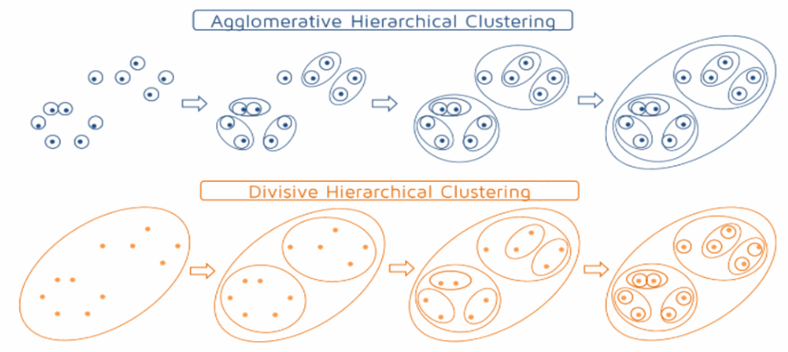
\includegraphics[width=\textwidth]{figures/6/hierarchical_clusterings}
	\caption{Hierarchical Clustering}
	\label{fig:hierarchical-clusterings}
\end{figure}

\section{Linkage}\label{sec:linkage}
\begin{description}[font=\emph]
	\item[Single Linkage] uses the \emph{smallest distance between all pairs} of data points in two clusters:
	\[ \data{ d(C, C') = \min_{x\in C, x{'}\in C{'}} d(x, x{'}) } \]
\end{description}


\end{document}